
%----------------------------------------------------------------------------------------
%	PACKAGES AND OTHER DOCUMENT CONFIGURATIONS
%----------------------------------------------------------------------------------------

\documentclass{article}

\usepackage{fancyhdr} % Required for custom headers
\usepackage{lastpage} % Required to determine the last page for the footer
\usepackage{extramarks} % Required for headers and footers
\usepackage{graphicx} % Required to insert images
\usepackage{mathtools, bm}
\usepackage{amssymb, bm}
\usepackage{graphicx}
\usepackage{algorithmic}

% Margins
\topmargin=-0.45in
\evensidemargin=0in
\oddsidemargin=0in
\textwidth=6.5in
\textheight=9.0in
\headsep=0.25in


\linespread{1.1} % Line spacing

% Set up the header and footer
\pagestyle{fancy}
\lhead{\hmwkAuthorName} % Top left header
\chead{\hmwkClass\ (\hmwkClassInstructor\ \hmwkClassTime): \hmwkTitle} % Top center header
\rhead{\firstxmark} % Top right header
\lfoot{\lastxmark} % Bottom left footer
\cfoot{} % Bottom center footer
\rfoot{Page\ \thepage\ of\ \pageref{LastPage}} % Bottom right footer
\renewcommand\headrulewidth{0.4pt} % Size of the header rule
\renewcommand\footrulewidth{0.4pt} % Size of the footer rule

\setlength\parindent{0pt} % Removes all indentation from paragraphs

%----------------------------------------------------------------------------------------
%	DOCUMENT STRUCTURE COMMANDS
%	Skip this unless you know what you're doing
%----------------------------------------------------------------------------------------

% Header and footer for when a page split occurs within a problem environment


% Header and footer for when a page split occurs between problem environments
   
%----------------------------------------------------------------------------------------
%	NAME AND CLASS SECTION
%----------------------------------------------------------------------------------------
\newcommand{\logoepfl}{
  \begin{center}
    
\includegraphics[width=4cm]{epfl.jpg}
  \end{center}
  \vspace{0.3cm}
  \hrule
}
\newcommand{\logolasec}{
  \vspace{1cm}
  \hrule
  \begin{center}
    
\includegraphics[width=4.5cm]{logo_lasec.jpg}
  \end{center}
}
\newcommand{\hmwkTitle}{Bachelor Project\ \#1} % Assignment title
\newcommand{\hmwkDueDate}{Spring 2016} % Due date
\newcommand{\hmwkClass}{IN, LASEC} % Course/class
\newcommand{\hmwkClassTime}{} % Class/lecture time
\newcommand{\hmwkClassInstructor}{Pr. Serge Vaudenay} % Teacher/lecturer
\newcommand{\hmwkAuthorName}{Max Premi} % Your name

%----------------------------------------------------------------------------------------
%	TITLE PAGE
%----------------------------------------------------------------------------------------
\title{
\logoepfl
\vspace{2in}
\textmd{\textbf{\hmwkClass:\ \hmwkTitle}}\\
\normalsize\vspace{0.1in}\small{Due\ on\ \hmwkDueDate}\\
\author{\textbf{\hmwkAuthorName}}
\vspace{0.1in}\large{\textit{\hmwkClassInstructor\ \hmwkClassTime}}
\vspace{3in}
\logolasec
}

%----------------------------------------------------------------------------------------

\begin{document}

\maketitle

\newpage
\section*{Abstract}
\addcontentsline{toc}{section}{Abstract}
The author takes the previous paper about a new Ciphertext-only Attacks on Hill Cipher, and try to improve it's complexity to get a better result than $O(d13^d)$.\\
${}$\hspace{1em}The goal of this project is to actually study the algorithm to recover the key matrix modulo 2 and then to improve the algorithm to get the key matrix modulo 26.\\
${}$\hspace{1em}The project report is organized as follows:Section 1 presents the Hill Cipher and the work done in the previous report. In Section 2, the author studies the the algorithm and try to improve the complexity to get the key matrix modulo 26. Section 3 presents the possible enhancement of the FFT of Algorithm 1. Experimental results and algorithms are presented at the end.
%----------------------------------------------------------------------------------------
%	TABLE OF CONTENTS
%----------------------------------------------------------------------------------------

\newpage
\tableofcontents
\newpage


%----------------------------------------------------------------------------------------
%	BEGIN OF REPORT
%----------------------------------------------------------------------------------------

\section{Introduction}
The motivation of this project is, first and foremost, to improve the Linear Cipher only attack on the Hill Cipher, by changing the recovering of the key modulo 26 and then look at the possible algorithm to improve the FFT in the recovery algorithm of matrix key modulo 2.\\
\\
Hill is a polygraphic substitution cipher based on linear algebra, invented by Lester S. in 1929. Each letter is represented by a number modulo 26, from $A=0$ to $Z=25$. The algorithm breaks the plaintext into blocks of size $d$ and then applies a key matrix $d \times d $ to these blocks to yield ciphertext blocks.\\
In order to encrypt a message, the ciphertext is calculated as a matrix product of the key and plaintext:

$$Y=K \times X$$

And in order to decrypt, we simply use linear algebra properties and multiply the cipher by the inverse of the key matrix.

$$X = K^{-1} \times Y$$

As it's a linear encryption, it can be simply broken with Known PlainText Attacks.\\
Indeed, it is known that a brute force attack can be done on this cipher, by intercepting $d^2$ plaintext/ciphertext character pairs, however to have a better complexity and less restrictive resources, improvement have been made to this simple brute force attack.\\
The attack described previously can determine the secret key almost uniquely if the length of ciphertext is at least $n =1.27d^2 [1].$\\ 
Later, it has been proved that it is possible to get the key matrix K, with minimum length of ciphertext required $n =8.96d^2 -O(\log d)$ [1].\\
This method has been then enhanced [1] using the divide-and-conquer technique, by eliminating repeated calculation while doing matrix multiplication, and have led to a ciphertext required length of $n=8,96d^2$. Eventually, using the Chinese Remainder Theorem [1], the length has been brought to $n=12.5d^2$, and the complexity to $O(d13^d)$.\\
By this same Chinese Remainder theorem, it is believed that we can find the key matrix modulo 2 first and then recover the matrix modulo 26 with a lower complexity [2].\\
It is shown in the previous paper that this matrix modulo 2 can be found in $O(d2^d)$, and the key matrix modulo 26 in $O(8^{nd})$.\\
\\
Let's briefly recall how this attack works:\\
If we consider $X$ a random vector constituted of $d$ letters, then we can pick a fixed vector $\lambda \in \{0,1\}^*$ and do the dot-product $\lambda \cdot X$ in $\mathbb{Z}/2\mathbb{Z}$.\\
The $d$ vectors $\lambda$ with largest non-trivial bias are obtained when $weight(\lambda) = 1$, and are used from now on for all computations.
Then with the aid of the bias($X$)= $\varphi_{X}(\frac{2\pi}{p})$ in $\mathbb{Z}/26\mathbb{Z}$, we find correspondence between $\lambda$ and $\mu$ (the last is the same vector but for ciphertext). More precisely we find correspondence between bias($\lambda \cdot X$) and bias($\mu \cdot Y$) and get $ \mu = (K^T)^{-1} \times\lambda $.\\
With this result and the approximation of all vectors $\mu$ via $S_n = \sum_{k=1}^{n}{(-1)^{\mu \cdot Y_{k}}}$, we recover the vectors column of the key matrix in ${Z}/2\mathbb{Z}$.\\
An algorithm using the correlation between vectors is used to identify the last one and first one easily, and then recursively sort all the vectors in the correct order.\\
All this process is described by algorithm 1 in the Appendix, and is done in time $O(d 2^d)$\\
\\
This project will present possible improvements of this algorithm to get a lower complexity than the one mentioned before, with the help of Sparse Fourier Transform. However, we first need to deal with the improvement for translation of key matrix from $\mathbb{Z}/2\mathbb{Z}$ to $\mathbb{Z}/26\mathbb{Z}$


\section{Key recovery modulo 26}
So now that we have the key matrix in $\mathbb{Z}/2\mathbb{Z}$, we can get the plain text in $\mathbb{Z}/2\mathbb{Z}$ using the linearity of the cipher.\\
To recover the key matrix in $\mathbb{Z}/26\mathbb{Z}$, we can use the Chinese Remainder Theorem, but we would get a complexity proportional to $O(13^d)$. In the previous paper, it was believed that it's possible to get the key matrix in $\mathbb{Z}/26\mathbb{Z}$ without considering $\mathbb{Z}/13\mathbb{Z}$.\\
First of all, we create a hash table using a very long text, and search mapping between segments of reference text and plain text modulo 2.\\
\#(seg in reference) = len(reference text) - $n +1$, with $n$ the segment size.\\
Indeed, if the following text is taken as an example: $thisisatest$, with $n$ = 5, we get the following segment:\\
 $ thisi, hisis, isisa, sisat, isate, sates, atest $ which is 7 segments $ 11 - 5 + 1 = 7 $\\
It's the same idea for \#(seg in plain) $= len(plain text) - n +1$, with $n$ the segment size.\\
\paragraph{Assumption 1.}\textit{All segments of length $n$ are independent with the same distribution}
\paragraph{Theorem 1.}\textit{R\'enyi entropy of order $\alpha$ where $\alpha \geq 0$ and $\alpha \neq 1$}:
\\
Let $a$, $b$ be random segment of length $n$ and $X$ the plaintext. We use R\'enyi entropy, with the following formula:\\
$$H_{\alpha}(X) = \frac{1}{1-\alpha}\log_{2}(\sum_{i=1}^{n}{\Pr(X=i)^{\alpha}})$$ 
When $\alpha = 2$, the following result is obtained:
$$H_{2}(X) = -\log_{2}(\sum_{i=1}^{n}{\Pr(X=i)^{2}})$$ that gives us the probability that a segment equals another one as $\sum_{i=1}^{n}{\Pr(X=i)^{2}} =\Pr(a=b)$.\\
The R\'enyi entropy represents more generally the quantity of information in the probability of a random variable's collision.\\
\\
Then we define good matching:segments are equal before and after modulo 2; and bad matching:segment which are not equal but equal modulo 2.\\
${}$\hspace{1em}For good matching, we have $E(\#$ good matching$) = (\# $segments in reference$) \times (\#$segment in plaintext$) \times 2^{-H_{2}(X)}$, as the number of good matching is actually the collision between segment in plaintext and segment in reference text multiplied by the R\'enyi entropy of this segment (which represents the rate of collision for a given block X).\\
Then the same is done for  $E(\# all matching)$, the difference is that we are in $\mathbb{Z}/2\mathbb{Z}$:$E(\#$ all matching$) = (\# $segments in reference$) \times (\#$segment in plaintext$) \times 2^{-H_{2b}(X \bmod 2)}$. And indeed it is understandable that if 2 words modulo 2 are equal, these words are not always equal modulo 26.\\
\\
As we consider independent letters in segment, the probability to find two of the same segment, with following occurrence of letters:$p(A)=0.0808$, $p(B)=0.0167$, ...etc, is:$\Pr(a=b)=((0.0808)^{2} +(0.0167)^{2} + ...)^{n} =0.06609^{n}$. Then $H_{2}(X) = -log_{2}0.06609^{n}$. The frequencies given in [8] are used as reference.\\
\\
${}$\hspace{1em}Now let's consider $E(\#$ all matching). As only 2 values are possible it's easier than the previous, indeed $E(\#$ all matching$) =(\# $segments in reference$) \times (\#$segment in plaintext$) \times 2^{-H_{2}(X \bmod 2)}$.\\
$H_{2}(X \bmod 2) = -\log_2(\sum_{i=0}^{1}{\Pr(X \bmod 2 =i)^2})$, where $\Pr(X \bmod 2=i)$ declined in $\Pr(X \bmod 2=0)$ and $\Pr(X \bmod 2 =1)$\\
From the experiment, we always get $0.5^n$ for $X \bmod 2$ so E(\# all matching) is never supposed to be different than $(\# $segments in reference$) \times (\#$segment in plaintext$) \times 0.5^n$.\\
\\
Then to have an idea of the distribution of good matching and bad matching, the ratio $\frac{E(\# \text{good matchings})}{E(\# \text{all matchings})}$ is computed: $\frac{E(\# \text{good matchings})}{E(\# \text{all matchings})} = \frac{|\text{segments in reference}| \times |\text{segment in plaintext}| \times 2^{-H_{2}(X)}}{|\text{segments in reference}| \times |\text{segment in plaintext}| \times 2^{-H_{2}(X \bmod 2)}}  = \frac{0.06609^n}{0.5^n} = \frac{1}{7.56^n} \cong \frac{1}{8^n} $\\
\\
To decrease the actual complexity, we need to increase the ratio of good matching as $E(\#$ all matchings$)$ can't be changed. So the only solution left is to try different assumptions and calculations for $E(\# $good matchings$)$.\\
\\
An interesting case is to consider blocks of letters as being independent from each others, and look at the evolution of the ratio through the growing block size. This is done in Experiment 2.\\
We take a very long sample text, and count heuristically the number of good and all matching. 
We finally conclude that it's possible to have a correct ratio for large size block, but as the actual algorithm depends too much on the blocksize, it is therefore impossible to get a correct complexity. For example, $blocksize=27$ gives ratio $\frac{1}{5}$ but still $\frac{1}{ratio^{blocksize}}$ is too high as $blocksize = 27$.
Eventually, the following parts focus on other way to implement this key matrix recovery modulo 26.\\

\section{Study of Algorithm to get $K_{26}$}
We are going to try to improve the complexity of algorithm 2 to find another complexity than $O(8^{nd})$ with $n$ the segment size and $d \times d$ the matrix size.\\
We want to turn the problem in another way, meaning instead of looking at all possible matching and do all the decryption possible with $d$ matching, try to find  the number of good matching we need so that an algorithm can find the key matrix by solving equations.\\
So the problem can be turned like this:find the number $y$ of matching needed to have a set of linear equation of the first order, to find the matrix coefficient in $\mathbb{Z}/26\mathbb{Z}$.\\
\subsection{Computation with conditional entropy}
What one can do, is taking the conditional entropy on the result of $X \bmod 2$.\\
\paragraph{Theorem 2.}\textit{Conditional R\'enyi entropy of order $\alpha$ where $\alpha \geq 0$ and $\alpha \neq 1$}:
$$H_{\alpha}(X \mid X \bmod 2 = y) = \frac{1}{1-\alpha}\log_{2}(\sum_{i=1}^{n}{\Pr(X=i \mid X \bmod 2= y )^{\alpha}}) , y \in \{0,1\} $$\\
For $\alpha = 2$, $H_{1}(X \mid X \bmod 2 = y) = -\log_{2}(\sum_{i=1}^{n}{\Pr (X=i \mid X mod2 = y)^{2}})$\\
In the case of single independent letter, the entropy declines into 2 possibilities, $H_{2}(X \mid X \bmod 2 = 0) $ and $H_{2}(X \mid X \bmod 2 = 1)$. The conditional probability is as following:
$$\Pr (X=i \mid X \bmod 2 = 0 ) = \frac{\Pr(X \bmod 2 = 0 \mid X = i) \Pr(X=i)}{\Pr(X \bmod 2 =0)} = $$
\[ \begin{cases}
      \frac{\Pr(X=i)}{\Pr(X \bmod 2 =0)} $$ & if \Pr(X \bmod 2 =0| X=i) \neq 0 \\
      0 & else
   \end{cases}
\]
and of course the same goes for 1.\\

Therefore, $\sum_{i=1}^{n}{(\Pr (X=i \mid X \bmod 2 = 0))^{2}} = ((\frac{\Pr(X=A)}{\Pr(X \bmod 2 = 0)})^{2} + (\frac{\Pr(X=C)}{\Pr(X \bmod 2) = 0})^{2} + ... )= 0.112$ , where $p(A)=0.0808 , p(B)=0.0318 , ...$  we get the probability from [8] exactly like the previous section.
And $\Pr(X=i \mid X \bmod 2 = 1) = 0.128$\\
We can now estimate the good matching by "class" of reduction modulo 2
Experiment 3 gives more details about the consideration of blocks instead of independent letters.
We can now get the ratio $\frac{E(\# \text{good matchings})}{E(\# \text{all matchings})}$ in class of modulo 2 reduction, so the conditional Expected value is as followed: $\frac{E(\# \text{good matchings} \mid X \bmod 2 = y)}{E(\# \text{all matchings} \bmod 2 = y)}$ or more clearly $\frac{E(\# \text{good matchings} \mid X \text{in class y})}{E(\# \text{all matchings in class y})}$. But in one class all the blocks are matching modulo 2 so it just gives $\Pr(\# \text{good matchings} \mid \text{X in class y})  = \Pr (X=i \mid X \bmod 2 = y) $\\
\\
Let's now try to resolve the number of equations needed so that we can resolve the key matrix modulo 26.\\
We get the cipher with the formula $ K \times X = Y$ , if we get $n$ good matching , $ K \times $  $\begin{pmatrix}
  - \\
  - \\
  ... \\
  a \\
	b\\
	c\\
	d\\
 \end{pmatrix} $
 = $\begin{pmatrix}
  u \\
  v \\
  ... \\
  - \\
	-\\
	-\\
	-\\
 \end{pmatrix}$
where $ u , v , ... $ represent the $n$ good matching and the $d-n $ others are not.\\
For this to work we need $d-n < n $ meaning $n > \frac{d}{2}$\\
If we call $N$ the number of matching, and $N_{good}$ the number of good matching.\\
We get $2n-d$ equations in $d^2$ unknowns.
What is the require number $N$ of matching to be sure that we can compute the matrix?\\
If $ \frac{d}{2} < n \leq d $ then we got the following:

$${N \choose N_{good}} \frac{13^{d^{2}}}{13^{2n-d N_{good}}} <  N^{N_{good}} \frac{13^{d^{2}}}{13^{2n-d N_{good}}}$$
That gives, considering that $N = r N_{good}$: $N_{good} > \frac{d^{2} \ln(13)}{(2n-d)\ln 13 - \ln r - \ln N_{good}}$\\
Now if $n>d$ then: 
$${N \choose N_{good}} \frac{13^{d^{2}}}{13^{d N_{good}}} <  N^{N_{good}} \frac{13^{d^{2}}}{13^{d N_{good}}}$$
Again as $N = r N_{good}$ we get: $N_{good} > \frac{d}{1-\frac{\ln r}{d \ln 13}}$\\
\\
From this we can say that $N_{good}$ must be bigger than $d$ , so we will take for simplification $N_{good} > 2d$\\

Thanks to the conditional entropy, we now know that some classes have a really good ratio of good matching/all matching. For example if $d=16$, we can try the following:\\ 
From the previous computation we need $N_{good} > 2d $, for blocksize 16. The ratio is 0.68 and so the number $N$ of matching will be : $ \frac{(2d+1)100}{68}$. If we apply the algorithm from the previous paper, which is in the Appendix, we can have correct result. IT takes $d$ matching from the list, here the class whith the better ratio, and would itterate =$\frac{1}{ratio^d} = 1.47^d = 1.47^{16}$ times. But is this class of matching enough to make the number of iteration needed to decrypt? Also this only works for $d>12$.



\section{Study of Faster Fourier Transform for Algorithm 1}
When a fast Fourier Transform (FFT) is applied to a signal of size $N$, the complexity in time is $O(N\log N)$.\\
A general algorithm for computing a DFT must take time proportional to its output size N. However, in some cases, most of the Fourier coefficients of a signal are small or equal to zero, meaning, the output of the DFT is sparse.\\
For sparse signals, the $n$ lower bound for the complexity of DFT no longer applies. If a signal has a small number $k$ of non-zero Fourier coefficients the output of the Fourier transform can be represented succinctly using only $k$ coefficients.\\
Hence, we can find Fourier Transform algorithm whose run time is sub-linear in the signal size $N$.\\
What we want is to enhance the possible FFT on a table called $n_y$ which contains the number of times $k$ where each cipher $Y$ appears. So it is a table containing numbers $\in \mathbb{N}$ of size $N=2^d$.\\

\subsection{Simple and practical algorithm for sparse Fourier transform}
This algorithm considers a complex vector $x$ of length $l$.\\
It computes the $k$-sparse Fourier transform in $O(\sqrt{kl}\log^{3/2}l)$, if $x$ is sparse then to find it takes exactly $O(klog^{2}l)$, but in general to estimate $x$ takes approximately $O(\sqrt{lk})$\\
So this algorithm is better if the ratio $\frac{l}{k} \in [2 \times 10^3, 10^6]$, but it's clearly not the best one as recently found are supposed to find it in a lower complexity ($k\log(l)$).\\
Now let's consider the input of this DFT to be $n_y$ with size $2^d$. This table contains integer whose sum is equal to the number of cipher given. As a result, we can't say that the resulting DFT of this vector will be sparse or not.

\subsection{Deterministic Sparse Fourier Approximation via Fooling Arithmetic Progressions}
This is also an SFT algorithm, meaning that it'll output the $k$-non null coefficient of the matrix. To do so you need to give it a threshold $\tau \in (0,1]$ and an oracle access to a function f, it outputs the $\tau$-significant Fourier Coefficient. It runs in $\log(N),\frac{1}{\tau}$.\\
An oracle access to a function take as input $x$ and return the $f(x)$ of the function $f$. A $\tau$-significant Fourier Coefficient is a coefficient whose magnitude is at least a $\tau$-fraction of the sum of squared Fourrier Coefficient
This algorithm is robust to random noise and local (meaning it runs in polynomial time).\\
\\
It's based on partition of set by binary search, we have at the beginning 4 intervals, an we're testing for the first two if the norm of $\hat{f}$ the Fourier Transform squared is equals to the $set_i$ oracle output squared.\\
Meaning more explicitly : $\hat{f}(J_i)^2 = \sum_{\alpha \in J_i}{|\hat{f}(\alpha)|^2}$. If this pass, it will output yes, and we'll be able to continue the algorithm by replacing the J and insert the $J_i$\\
The heart of the code is actually to decide which intervals potentially contain a significant Fourier coefficient. Yes if weight on $J$, exceeds significant threshold $\tau$, NO if J larger.\\
The threshold $\tau$ can be chosen, with the fact that a $\alpha$ is a $\tau -significant$ Fourier coefficient iff $|\hat{f}|^2 \geq \tau||f||^{2}_2$\\ where $\hat{f} = \langle f,X_{\alpha} \rangle$ and $X_{\alpha} = e^{2\pi i \alpha x/N}$.\\
Considering the table $n_y$ of size $2^d$, we get $\tau||f||^{2}_2 < \tau \times n^2$ as there are $n$ ciphers were $2^d <n$. So the semi-norm will be the smallest if they are all distributed equally in the "buckets". That gives approximately ${\lfloor \frac{n}{2^d} \rfloor}^{2}$ ciphers by buckets, and the worst case where the semi norm is the bigger is when all ciphers are in one place meaning $n^2$.\\
Let's take the value from the example of the previous paper: 6200 ciphers and blocksize =10. There for the best case, i.e, all equally distributed each bucket contains ${\lfloor \frac{6200}{2^{10}} \rfloor} = 6$, we get $|\hat{f}|^2 \geq \tau||f||^{2}_2 =  6144^2 \geq \tau 36864$ , where 6024 is the biggest Fourier coefficient and all the others are 0 so $ 1 = \tau$ that will be a good result but the probability that it arrives is clearly too small to be considerate.\\
For the worst case we would get:$|\hat{f}|^2 \geq \tau||f||^{2}_2 =  \alpha \geq \tau 6200^2$ where $\alpha$ is one of the smallest coefficient but still bigger the order $10^1$  
The problem is that $\tau$ will need to be very big to match the previous inequality. So the complexity will depends on $\frac{1}{\tau}$ and it'll clearly be too important to be considered.\\

\subsection{Nearly optimal Sparse Fourier Transform}

We want here to compute the $k$-sparse approximation to the discrete Fourier transform of an $2^d$-dimensional signal.\\
In the case where the input has at most $k$ non-zero Fourier coefficient, we got $O(k.\log(2^d))$ time, else we have $O(k.\log(2^d).\log(\frac{2^d}{k}))$\\
The basis is still the same, if a signal has a small number $k$ of non-zero Fourier coefficient, the output of this DFT can be represented succinctly using only $k$ coefficient.\\
What is required, is that the input size $n$ is a power of 2 which is complete in this case.\\
This algorithm has a better performance if and only if $ k < O(\frac{2^d}{\log(2^d)}$. This won't be the case here and the formula for the $k$ superior to this limit perform too poorly for worst case:$O(\sqrt(2^d k) \log^{\frac{3}{2}}(2^d))$


\section*{Experiment}
\addcontentsline{toc}{section}{Experiment}
\subsection*{Experiment 1:Probability of independent English letters}
\addcontentsline{toc}{subsection}{Experiment 1:Probability of independent English letters}
From the frequency letter given by Wikip\'edia, in english we got the following result :\\
Probability summed = 0.9999999999999999
\\
Sum of probability squared = 0.06549717159999999, which corresponds to $(\sum_{i=0}^{25}{\Pr(i=y)^2})^n, y \in \{alphabet\} $\\
Sum of probability that gives 0 modulo 2 squared  = 0.32298762240000006 which corresponds to $(\sum_{i=0}^{25}{\Pr(i=0)^2})^n, i \in \{alphabet \bmod 2\} $\\
Sum of probability that gives 1 modulo 2 squared = 0.18634762239999997 which corresponds to $(\sum_{i=0}^{26}{\Pr(i=1)^2})^n, i \in \{alphabet \bmod 2\} $\\
Ratio of good matching and all matching=$0.1285934407027314^n$\\
From the R\'enyi entropy seen previously we get, $\frac{|\text{segments in reference}| \times |\text{segment in plaintext}| \times 2^{-H_{2}(X)}}{|\text{segments in reference}| \times |\text{segment in plaintext}| \times 2^{-H_{2}(X \bmod 2)}}  = \frac{0.06549^n}{0.5^n} = \frac{1}{7.776^n}$
So $\frac{1}{7,77644^n}$ which match the result found.
\\
\\
Another site [8], with a total number of $100000$ letters composed with texts from Edgar Allan Poe, Arthur Conan Doyle, and 4 articles from encyclopedia Encarta 95:\\
\\
Probability summed = 0.9999000000000001\\
Sum of probability squared = 0.06609151 which corresponds to $(\sum_{i=0}^{25}{\Pr(i=y)^2})^n, y \in \{alphabet\} $\\
Sum of probability that gives 0 modulo 2 squared = 0.32001649 which corresponds to $(\sum_{i=0}^{25}{\Pr(i=0)^2})^n, i \in \{alphabet \bmod 2\} $\\
Sum of probability that gives 1 modulo 2 squared = 0.18852964 which corresponds to $(\sum_{i=0}^{25}{\Pr(i=1)^2})^n, i \in \{alphabet \bmod 2\} $\\
Ratio of good matching and all matching=$0.12996168115565054^n$\\
From the R\'enyi entropy seen previously we get, $\frac{|\text{segments in reference}| \times |\text{segment in plaintext}| \times 2^{-H_{2}(X)}}{|\text{segments in reference}| \times |\text{segment in plaintext}| \times 2^{-H_{2}(X \bmod 2)}}  = \frac{0.06609^n}{0.5^n} = \frac{1}{7.69n}$
So $\frac{1}{7,69457^n}$ which also match what we expected.

\subsection*{Experiment 2:Probability considering blocks of size $d$}
\addcontentsline{toc}{subsection}{Experiment 2:Probability considering blocks of size $d$}
So calculation are done on a text of approximately $860000$ characters to see the evolution of the ratio good matching/bad matching.\\
A program is ran to see the evolution for a block size between 1 and 25, and give the ratio, thanks to the probability that a block appears. It is completely heuristic as it's just counting the number of block that appears and do base all computation on the number of time it appears.
So the basic is to choose a blocksize, then it'll count every different blocks that appears modulo 26 and also convert them in modulo 2.
Then it'll compute the probability that a good matching appears with the following : $\sum_{X \in block}({\frac{\#X -1}{\#block -1}})^2 $\\
The exact same thing is done with X in modulo 2, to get the probability of all matching, and then we compute the ratio $\frac{E(\# good matchings)}{E(\# all matchings)}$\\
With this, the evolution of the ratio in function of the block size looks like this:\\
\\
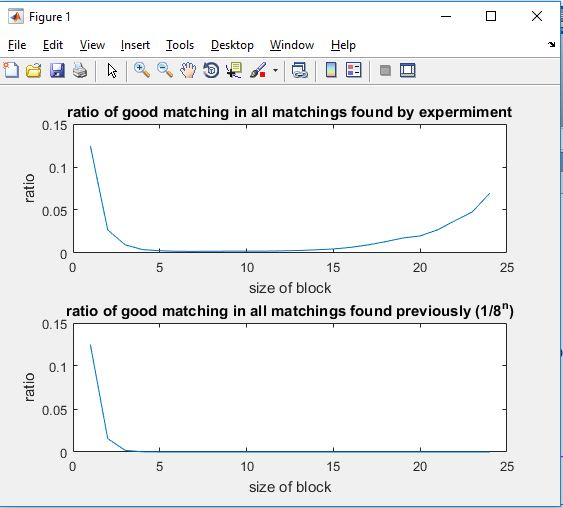
\includegraphics[width=90mm]{ratio.jpg}
So we can see that the ratio follow the $\frac{1}{8^n}$ until blocksize 15, then it goes up again to almost match 1/8 for blocksize 24. With the current algorithm and this size of block the number of iteration would be $8^d$ and as $d = 24$ is really large it's still not effective.\\
Even if the ratio do not behave as previously thought, the complexity stay too high for reasonable blocksize between 8 and 14, and if the blocksize is increased to a certain point, the ratio is good but the complexity depends on a ratio power the blocksize, so it will not be good enough to be taken in account.

\subsection*{Experiment 3:Conditional Probability considering that we know X mod 2}
\addcontentsline{toc}{subsection}{Experiment 3:Conditional Probability considering that we know X mod 2}
In this experiment, we still consider the text from the previous part and sort block of letter in class of reduction modulo 2.
For example the block $ab$ will be in the class $01$. From this sorting we can know which class has the best ratio of good matching.
We know select the best class as following\\
The best class is not the class that have the best ratio of good matching over all matching, as we can have a class where there is only 3 matching and 2 are equals. So to avoid classes like this we just take the class with the highest number of good matching.
To have an idea of the number of block, it is almost 847400.\\
\begin{tabular}{c|c|c|c|c}
  \hline
  blocksize & Best Class & Ratio of good matching & \# block from this class & Bigger blocksize\\
	1 & 0 & 0.119870 & 478261 & 478261\\
	2 & 11 & 0.062238 & 122847 & 246310\\
	3 & 110 & 0.033030 & 94719 & 151590\\
	4 & 1110 & 0.02486952 & 24273 & 81141\\
	5 & 10110 & 0.0098346 & 36098 & 48807\\
	6 & 011110 & 0.0360992 & 3300 & 25434\\
	7 & 1010001 & 0.00833618 & 10022 & 15094\\
	8 & 10100010 & 0.0199979 & 6219 & 8132\\
	9 & 100110101 & 0.03706977 & 3127 & 4544\\
	10 & 1001101010 & 0.075711852 & 2183 & 2514\\
	12 & 000110100010 & 0.1072417 & 654 & 784\\
	14 & 10101110100010 & 0.332720389 & 215 & 287\\
	16 & 1000010000100011 & 0.6810255 & 103 & 122\\
	\hline
\end{tabular}

\appendix
\newpage
\section*{Algorithm}
\addcontentsline{toc}{section}{Algorithm}
You hash a reference text.\\
You take the key matrix that you get from algorithm 1, find plain text in $\mathbb{Z}/2\mathbb{Z}$, and create an array.\\
find the list of all matching: find all pairs $(seg,str)$ such that $seg$ is a segment of plaintext modulo 2 and $str$ $\in hash(seg)$ and save it in a list.\\
\begin{algorithmic}[1]
	\REPEAT
\STATE select d matching from the list (you'll get a $d\times d$ key matrix)
\FOR{each of these matchings ($seg_{i}$, $str_{i}$)}
	\STATE extract $block_{i}$ from $seg_{i}$ and $str'_{i}$ from $str_{i}$,
	\STATE then find $ciphertext_{i}$ such that $K^{-1}$ x $ciphertext_{i}$ mod 2 = $block_{i}$
\ENDFOR
\STATE solve $ciphertext_{i} = K * str'_{i}$ for i=1 to d
\STATE compute $K^{-1} * $ciphertext
\UNTIL decryption make sense
\end{algorithmic}
number of iteration is $ \frac{1}{ratio^{nd}} = 8^{nd}$
\\
\\
The following algorithm is to recover the key matrix in $\mathbb{Z}/2\mathbb{Z}$\\
\begin{algorithmic}[1]
\STATE Part1:\\
\REQUIRE{Ciphertext $Y_1,Y_2,...,Y_n$}\\
\ENSURE{K($\bmod 2$)}\\
\FORALL{$\mu$}
	\STATE compute $S_n(\mu) = \sum_{y}{(-1)^{\mu.y} \times n_y}$ where $n_y=\#\{k;Y_k=y\}$
\ENDFOR
\STATE set all $\mu$ to the d values of $\mu$ with largest $S_n(\mu)=bias(\mu.Y)$
\STATE Part2:\\
\FORALL{$(i,i')$}
	\STATE compute $n_{00}(i,i')=\#\{k<n:(\mu_i .Y_k,\mu_i'.Y_{k+1})=(0,0)\}$
\ENDFOR
\STATE set $(i_d,i_1)$ to the first pair with lowest $n_{00}$
\\
\STATE Part3:\\
\FORALL{$t=2$ to $d-1$}
	\FORALL{i $\notin \{i_1,i_2,..,i_{t-1},i_d\}$}
		\STATE compute $n_{00}(i,i{'})=\#\{k:(\mu^{T}_{i_{t-1}}Y_{k},\mu^{T}_{i}Y_{k})=(0,0)\}$\\
	\ENDFOR
	\STATE take i such that $n_{00}$ is minimum and set $i_t=i$\\
\ENDFOR
\STATE set $\mu = (\mu_{i1},\mu_{i1},...,\mu_{id})$ and $K=(\mu^-1)^T$
\STATE output K
\end{algorithmic}
Here to be faster we store $n_y$ in a table and we do a FFT on this table to get $S_n$. With this operation the total complexity drop from $O(d^2 \times 2^d)$ to $O(d \times 2^d)$
But it seems with some other techniques we could do better.


\section*{References}
\addcontentsline{toc}{section}{References}
[1] S. Shazaei, S. Ahmadi. \textit{Ciphertext- only attack on} $d \times d$ \textit{Hill in} $O(d13^d)$.\\
\\[0pt]
[2] Alina, Matyukhina. \textit{Cryptanalysis of the Hill Cipher}.\\
\\[0pt]
[3] Akavia, A. \textit{Deterministic Sparse Fourier Approximation via Fooling Arithmectic Progressions}.\\
\\[0pt]
[4] Akavia, A., Goldwasser, S., Safra, S. \textit{Proving Hard-Core Predicates Using List Decoding}.\\
\\[0pt]
[5] Hassanieh, H., Indyk, P., Katabi, D., Price, E. \textit{Nearly optimal sparse Fourier transform}.\\
\\[0pt]
[6] Hassanieh, H., Indyk, P., Katabi, D., Price, E. \textit{Simple and practical algorithm for sparse Fourier transform}.\\
\\[0pt]
[7] Iwen, M.A. \textit{Combinatorial Sublinear-Time Fourier Algorithms}.\\
\\[0pt]
[8] http://www.nymphomath.ch/crypto/stat/anglais.html\\



\end{document}
